\chapter{Marco Metodológico}

\par En este capítulo se describirá la secuencia del algoritmo desarrollado para el cálculo de las variables por sección en el horno, haciendo referencia a los métodos y ecuaciones antes descritos. Finalizando con la descripción de la interfaz gráfica diseñada para introducir y mostrar los datos y resultados del simulador.

\section{Algoritmo}

\par El diagrama ilustrado en la Figura \ref{fig:diagrama-algo}, permite visualizar la secuencia del algoritmo y sera detallado en las subsecciones consiguientes.

\begin{figure}[hbt]
\begin{center}
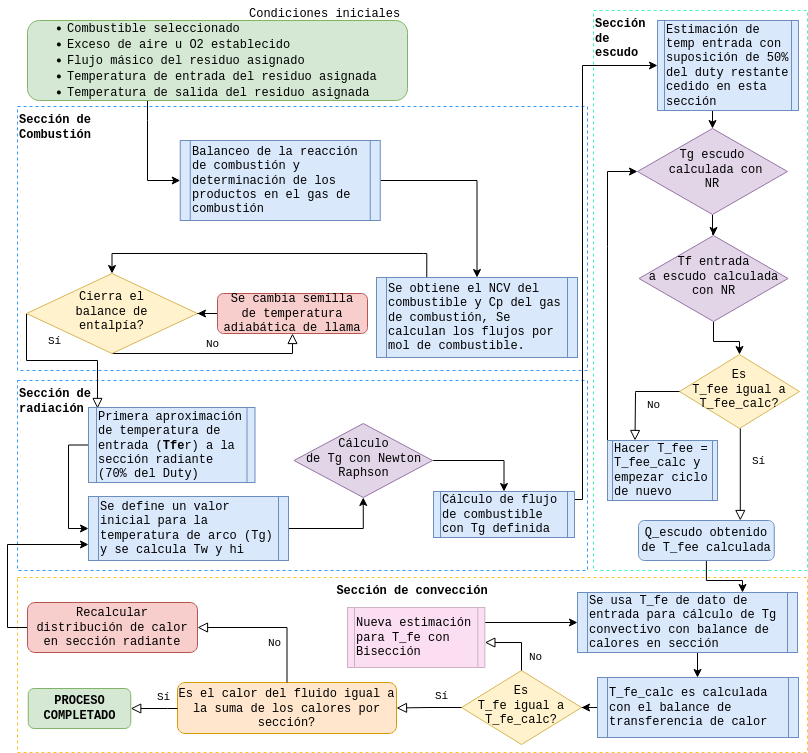
\includegraphics[scale=0.45]{images/diagrama-algo}
\caption[Diagrama de algoritmo]{Diagrama descriptivo del algoritmo desarrollo para el simulador.}
\label{fig:diagrama-algo}
\end{center}
\end{figure}

\subsection{Ciclo externo}

\par Este ciclo se encarga de recibir todos los parámetros de entrada y correr cada una de las siguientes subsecciones como funciones, es donde se define la distribución de calor entre las secciones del horno y varia este valor para alcanzar la tolerancia deseada con un método Newton Rapshon aplicado a la siguiente ecuación.

\begin{equation}
\label{eq:ciclo_externo}
\frac{(Q_{residuo} - Q_{calc})}{Q_{calc}} \approx 0
\end{equation}

donde:

\begin{gather*}
Q_{residuo} = Masa_{residuo} * Cp_{residuo} * {\Delta}T_{residuo} \\
Q_{calc} = Q_{radiante} + Q_{escudo} + Q_{convectivo} \\
Q = Calor o Duty
\end{gather*}

\par Lo que se traduce en que el calor absorbido por el residuo debe ser igual al calor suministrado en cada una de las secciones del horno.

\par El valor inicial de distribución radiante esta definido en 64\% y esta converge para el rango de temperaturas permitido en la interfaz del simulador. En las siguientes subsecciones se detallan las ecuaciones para cada etapa del horno.

\subsection{Combustión}

\par Esta sección del algoritmo esta encargada de calcular toda la energía que entra al horno

\subsection{Radiación}

\par 

\subsection{Escudo}

\par 

\subsection{Convección}

\par 


\section{Interfaz de usuario}

\par La interfaz fue desarrollada usando los lenguajes básicos de programación web, HTML CSS y JavaScript, lo que hace que sea totalmente editable y pueda correr en cualquier ordenador o dispositivo móvil con navegador web.

\subsection{Introducción de datos}

\par En esta sección se desarrollan dos vistas, una simplificada para introducir solo los datos más relevantes del proceso y que dirige a una pantalla de resultados donde se pueden comparar dos estados; otra donde se observan todas las variables que permite modificar el proceso y esta a su vez tiene dos opciones de resultados, una pantalla de valores numéricos detallados y una segunda pantalla que muestra una variación gráfica en el rango de cuatro variables a escoger.  

\subsection{Resultados ampliados}

\par En esta vista se detallan todas las variables resultantes por cada sección del horno, se puede escoger el sistema de unidades a expresarse en la pantalla anterior.

\subsection{Resultados comparativos}
\subsection{Gráficas de tendencias}
\subsection{Descripción de uso y alcances}